\newpage

\section{Symmetries}
\begin{definition}
A symmetry is a transformation that takes a figure onto itself.  
\end{definition}
\begin{prob}
List the symmetries of an equilateral triangle.  Explain how you know you have them all.  
\end{prob}

%%  Find symmetries in figures found on the Web.  Include Frieze patterns.  

\begin{prob}
Find some figures in section 1.2 of your text and describe the symmetries you notice.  Try to find reflection symmetry, rotation symmetry, and translation symmetry.  \fixnote{Insert pictures from Web.}
\end{prob}

\begin{prob}
Suppose the symmetries of a square are called $R_0$, $R_{90}$, $R_{180}$, $R_{270}$, $V$, $H$, $D$, $D'$, based upon the figure below.  
$$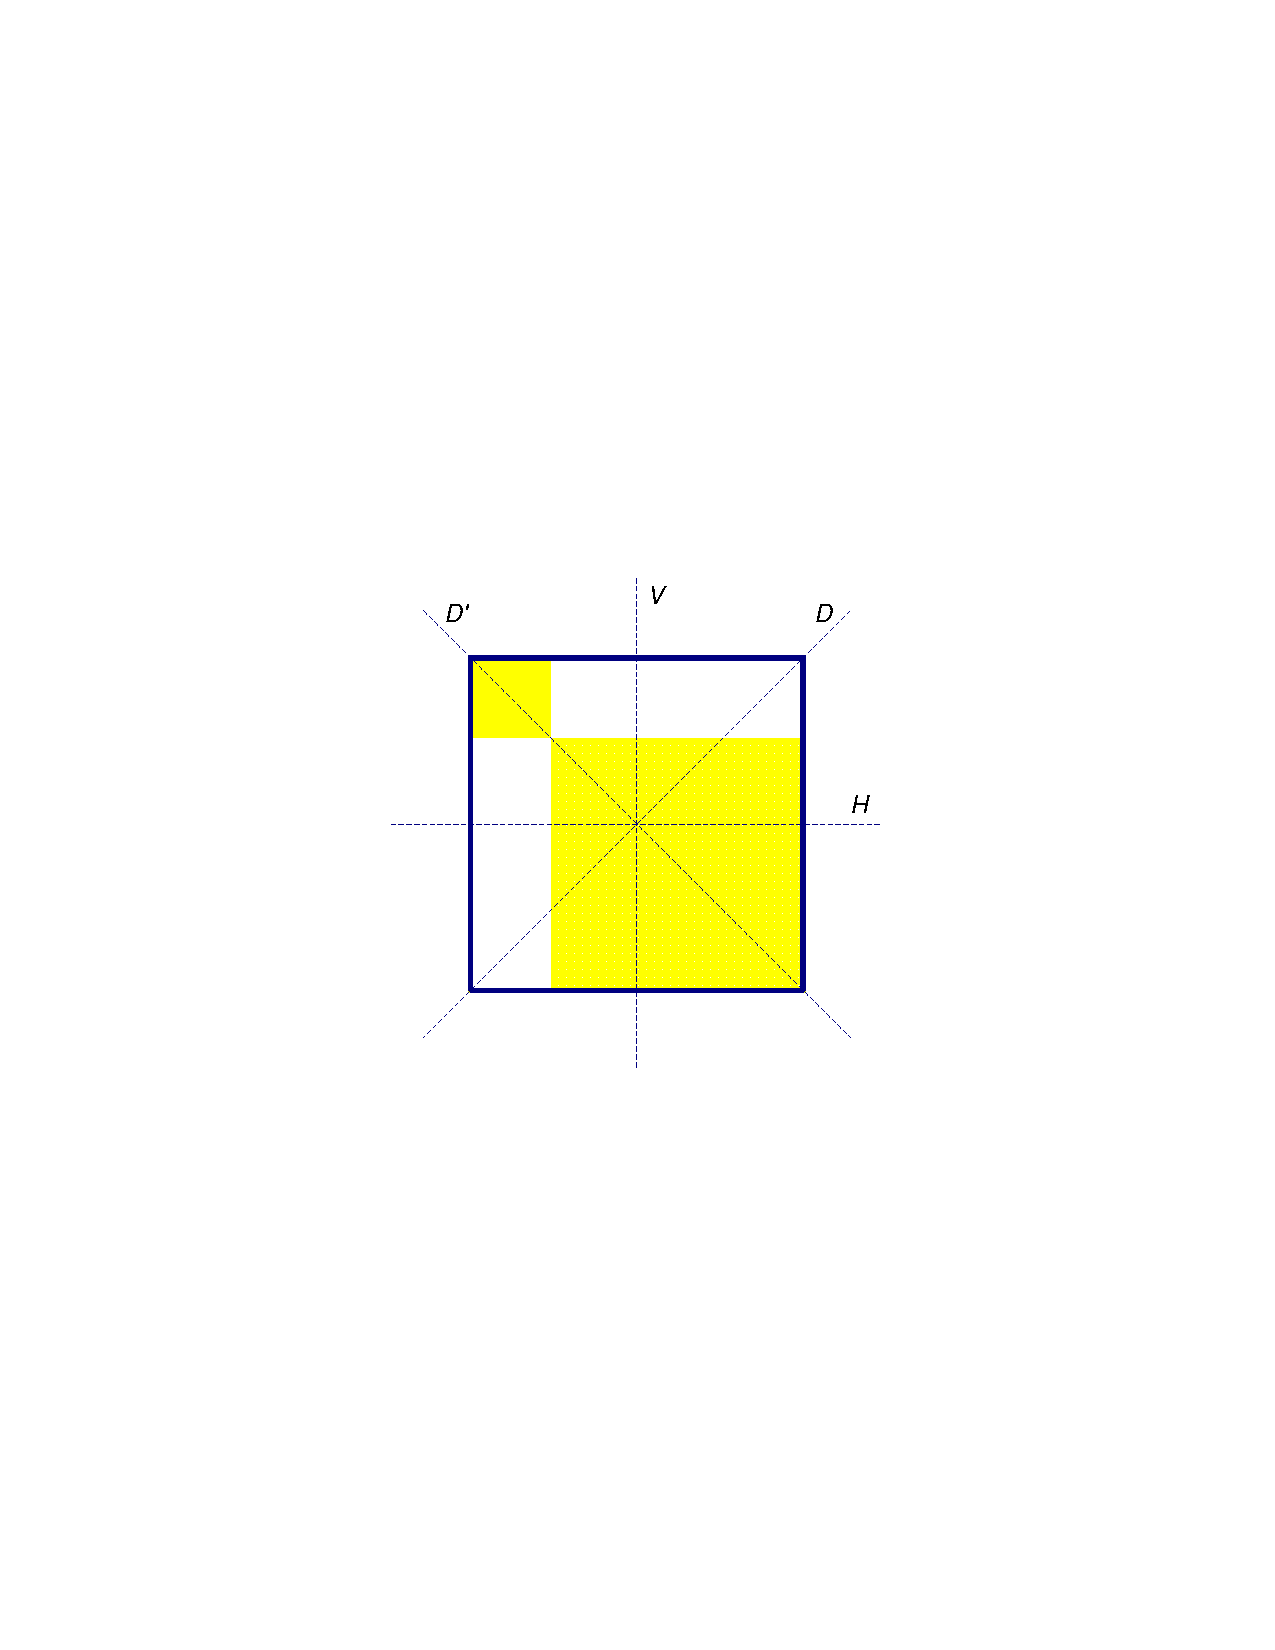
\includegraphics[scale=0.6]{../graphics/D4}$$
Hint:  To identify a single transformation that accomplishes a sequence of transformations, do the transformations physically with a square piece of paper marked with ``FRONT'' on the side that starts facing you.  Or mark the corners of the square with $A$, $B$, $C$, and $D$.  
\begin{enumerate}
\item Complete the following table, where the entry at (row, column) is the symmetry that results from the sequence of symmetries given by the row heading followed by the column heading.  
\item What patterns and not-quite-patterns do you notice in the table?  For example, which elements ``commute'' with which other elements?
\item What facts about isometries can you observe in the table?  For example, what can you say generally about sequences of rotations and reflections?  
\end{enumerate}

{\[\arraycolsep=12pt\def\arraystretch{3}
\begin{array}{|l||l|l|l|l||l|l|l|l|}
\hline
 & R_0 & R_{90} & R_{180} & R_{270} & V & H & D & D' \\ \hline\hline
R_0 & & & & & & & & \\ \hline
R_{90} & & & & & & & & \\ \hline
R_{180} & & & & & & & & \\ \hline
R_{270} & & & & & & & & \\ \hline\hline
V & & & & & & & & \\ \hline
H & & & & & & & & \\ \hline
D & & & & & & & & \\ \hline
D' & & & & & & & & \\ \hline
\end{array}
\]}
\end{prob}



